\documentclass[aspectratio=169 %可调屏宽比16:9(169),4:3(43)
,serif,mathserif]{beamer}

\mode<presentation>{
%\usetheme{default}
%\usetheme{AnnArbor}
%\usetheme{Antibes}
%\usetheme{Bergen}
%\usetheme{Berkeley}
%\usetheme{Berlin}
%\usetheme{Boadilla}
%\usetheme{CambridgeUS}
%\usetheme{Copenhagen}
%\usetheme{Darmstadt}
%\usetheme{Dresden}
%\usetheme{Frankfurt}
%\usetheme{Goettingen}
%\usetheme{Hannover}
%\usetheme{Ilmenau}
%\usetheme{JuanLesPins}
%\usetheme{Luebeck}
\usetheme{Madrid}
%\usetheme{Malmoe}
%\usetheme{Marburg}
%\usetheme{Montpellier}
%\usetheme{PaloAlto}
%\usetheme{Pittsburgh}
%\usetheme{Rochester}
%\usetheme{Singapore}
%\usetheme{Szeged}
%\usetheme{Warsaw}
% As well as themes, the Beamer class has a number of color themes
% for any slide theme. Uncomment each of these in turn to see how it
% changes the colors of your current slide theme.
%\usecolortheme{albatross}
%\usecolortheme{beaver}
%\usecolortheme{beetle}
%\usecolortheme{crane}
%\usecolortheme{dolphin}
%\usecolortheme{dove}
%\usecolortheme{fly}
%\usecolortheme{lily}
%\usecolortheme{orchid}
%\usecolortheme{rose}
%\usecolortheme{seagull}
%\usecolortheme{seahorse}
%\usecolortheme{whale}
%\usecolortheme{wolverine}
%\setbeamertemplate{footline} % To remove the footer line in all slides uncomment this line
%\setbeamertemplate{footline}[page number] % To replace the footer line in all slides with a simple slide count uncomment this line
%\setbeamertemplate{navigation symbols}{} % To remove the navigation symbols from the bottom of all slides uncomment this line
}
\usepackage{adjustbox}
\usepackage{indentfirst} 
\usepackage{amsmath, amsfonts, epsfig, xspace}
\usepackage{algorithm,algorithmic}
\usepackage{beamerthemesplit}
\usepackage{booktabs}
\usepackage{bm}
\usepackage{braket}
\usepackage{calligra}
\usepackage{color}
\usepackage[T1]{fontenc}
\usepackage{fontspec}
\usepackage{ctex}
\usepackage{latexsym}
\usepackage{multicol}
\usepackage{multimedia}
\usepackage{calligra} \DeclareMathAlphabet{\mathcalligra}{T1}{calligra}{m}{n} \DeclareFontShape{T1}{calligra}{m}{n}{<->s*[2.2]callig15}{}
\usepackage{pstricks,pst-node}
\usepackage{ragged2e}
\usepackage{setspace}
\usepackage[normal,tight,center]{subfigure}
\setlength{\subfigcapskip}{-.5em}
\setlength{\parindent}{2em}
\begin{document}
\title{Sound and Complete Neural Network Repair with Minimality and Locality Guarantees} % The short title appears at the bottom of every slide, the full title is only on the title page
\author[Chi~Zhiming]{Reporter:~Chi~Zhiming} % Your name
\institute[ISCAS] % Your institution as it will appear on the bottom of every slide, may be shorthand to save space
{	
	%Lanzhou University \\ % Your institution for the title page
	%\medskip
	%\textit{chizhm16@lzu.edu.cn} % Your email address
}
	\CTEXoptions[today=old]
	\date{\today} % Date, can be changed to a custom date
\begin{frame}[plain]\vspace{1.5em}
\titlepage\vspace{-0.5cm}
%\centerline{\includegraphics[height=0.30\textheight]{logo.png}}
%\hfill 指导教师:xxx
\end{frame}
\begin{frame}{目录}
\tableofcontents
\end{frame}
\AtBeginSection[]
{
\begin{frame}{\tiny}
\frametitle{目录}
\tableofcontents[currentsection]
\end{frame}
}
%----------------------------------------------------------------------------------------
%	PRESENTATION SLIDES
%----------------------------------------------------------------------------------------

%------------------------------------------------
\section{Introduction} % Sections can be created in order to organize your presentation into discrete blocks, all sections and subsections are automatically printed in the table of contents as an overview of the talk
%------------------------------------------------

\setbeamercovered{transparent} 
\begin{frame}{Contribution}
\begin{enumerate}
	\item The method is both sound and complete: the repaired network is guaranteed to fix the buggy input, and a patch is guaranteed to be found for any buggy input  \pause
	\item This approach preserves the continuous piecewise linear nature of ReLU networks. \pause
	\item It can also automatically generalizes the repair to all the points including other undetected buggy inputs inside the repair region, is minimal in terms of changes in the function space, and guarantees that outputs on inputs away from the repair region are unaltered. 	
\end{enumerate}
\end{frame}


\begin{frame}
	\frametitle{Existing network repair categories}
	\begin{itemize}
		\item Retraining\/fine-tuning:
		\begin{itemize}
			\item Retrain or fine-tune the network with the newly identified buggy inputs and the corresponding corrected outputs
			\item No guarantee, expensive and requires access to the original training data
		\end{itemize} \pause
		\item Direct weight modification:
		\begin{itemize}
			\item optimization or a verification problem
			\item optimization-based approach cannot guarantee removal of the buggy behaviors, 
			\item and the verification-based approach does not scale beyond networks of a few hundred neurons.
			\item both approaches suffer from substantial accuracy drops on normal inputs.
		\end{itemize} \pause
		\item Architecture extension:
		\begin{itemize}
			\item only work: PRDNN
			\item The decoupling causes the repaired network to become discontinuous (in the functional sense).
			\item It still cannot isolate the output change to a single buggy input from the rest of the inputs.
		\end{itemize}
	\end{itemize}
\end{frame}

\begin{frame}
	\frametitle{PRDNN}
	\begin{columns}
		\begin{column}{.38\textwidth}
			\begin{figure}[htbp]
				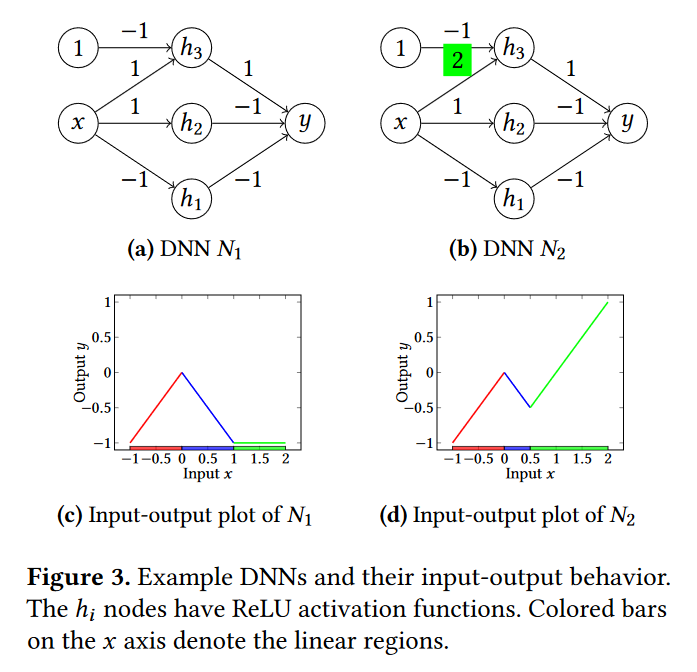
\includegraphics[width=\linewidth]{1.png}
			\end{figure}
		\end{column}

		\begin{column}{.65\textwidth}
			\begin{figure}[htbp]
				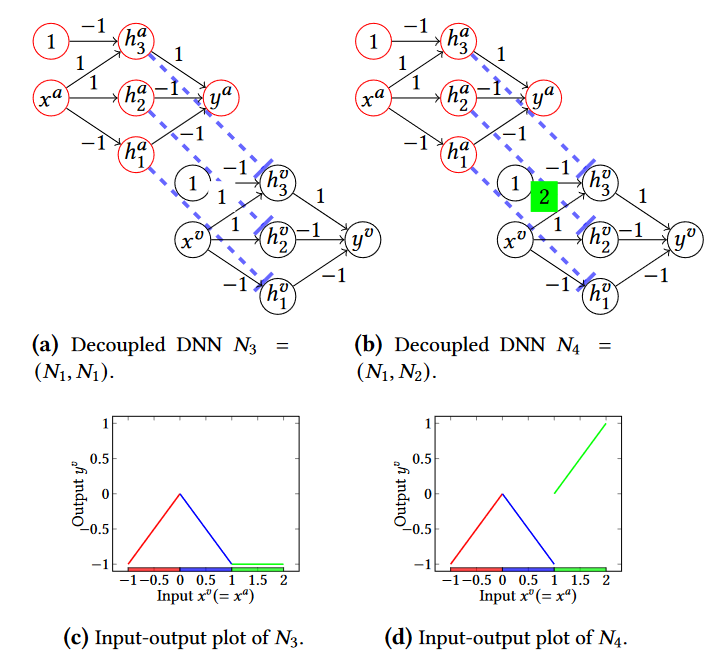
\includegraphics[width=.58\textwidth]{2.png}
			\end{figure}
		\end{column}
	\end{columns}
\end{frame}

\begin{frame}
	\frametitle{Common Problem: Modification are global}
	\begin{enumerate}
		\item This means that a correct behavior on another input, regardless of how far it is away from the buggy input, may not be preserved by the repair. \pause
		\item Worse still, the repair on a new buggy input can end up invalidating the repair on a previous buggy input. \pause
		\item Reason: It only poses a structural constraint, and does not limit the changes on the input-output mapping of the neural network.
	\end{enumerate}
\end{frame}

\begin{frame}
	\frametitle{Some Definition}
	\begin{itemize}
		\item Linear Regions:
		\begin{itemize}
			\item the set of inputs that correspond to the same activation pattern in a ReLU DNN $f$
			\item a convex polytope, in the input space $X$ on which $f$ is linear.
		\end{itemize} \pause

		\item Correctness Specification:
		\begin{itemize}
			\item $\Phi=\left(\Phi_{i n}, \Phi_{o u t}\right)$, $\Phi_{i n}$ is the union of some linear regions and $\Phi_{o u t}$ is a convex polytope.
		\end{itemize} \pause

		\item Repair:
		\begin{itemize}
			\item Area repair \& Point-wise repair
			\item Minimal repair: maximum distance between $f$ and $repair(f)$ over the whole input domain X
		\end{itemize} 
		% 这里缺了个pointwise repair 到 area repair 的转换,看看后面会不会补

	\end{itemize}
\end{frame}

\begin{frame}
	\frametitle{Repair Desiderata}
	\begin{enumerate}
		\item Preservation of CPWL.
		\item Sound and Complete.
		\item Generalization.
		\item Locality and Limited side effect. \pause
		\item Minimality: a significant departure from existing methods, that focus on minimizing the change in weights which has no guarantee on the amount of change in the function space.
	\end{enumerate}
\end{frame}

\section{Their Approach}
\begin{frame}
	\frametitle{Outline}
	\begin{itemize}
		\item Given a linear region $\mathcal{A}$, The approach is to synthesize a patch network $h_{\mathcal{A}}$ such that $\widehat{f}=f+h_{\mathcal{A}}$ and $\widehat{f} \models \Phi$, which has a combination of two sub-networks.
		\item A support network $g_{\mathcal{A}}$ which behaves like a characteristic function to ensure that $h_{\mathcal{A}}$ is almost only active on $\mathcal{A}$.
		\item An affine patch function network $p_{\mathcal{A}}(x)=\boldsymbol{c} x+d$ such that $\left(f+p_{\mathcal{A}}\right)=\Phi$ on $\mathcal{A}$.		
	\end{itemize}
\end{frame}

\begin{frame}
	\frametitle{Support Networks}
	\begin{itemize}
		\item This structure approximates the characteristic function, which are keys to ensuring localized repairs in our algorithm.
		\begin{figure}[htbp]
			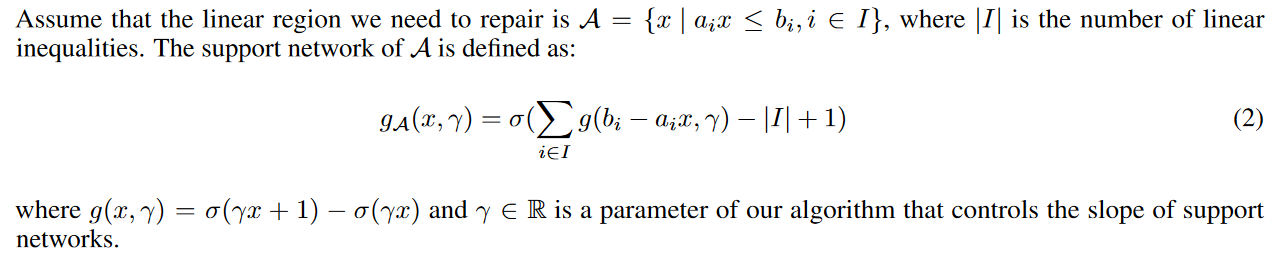
\includegraphics[width=1\linewidth]{3.png}
		\end{figure}
	\end{itemize}
\end{frame}

\begin{frame}
	\frametitle{Explanation of Support Networks}
	\begin{enumerate}
		\item Discontinuous $\to$ Continuous:
		\item \begin{figure}[htbp]
			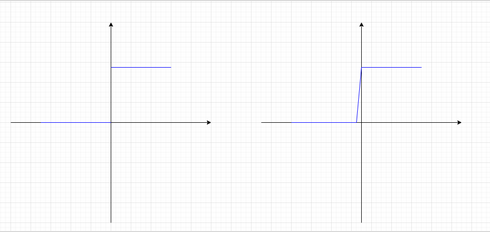
\includegraphics[width=.5\linewidth]{4.png}
		\end{figure}
		\item For $g(x, \gamma)=\sigma(\gamma x+1)-\sigma(\gamma x)$, if $0>x \geq -\frac{1}{\gamma}$, then $g(x, \gamma)=\gamma x+1$.
	\end{enumerate}	
\end{frame}

\begin{frame}
	\frametitle{Explanation of Support Networks}
	\begin{itemize}
		\item For $a_i x \leq b_i$, it has equivalent formula:
		\item \begin{equation}
			\lim\limits_{\gamma \to+\infty}  \gamma(b_i -a_ix) + 1 \geq 0 
		\end{equation}
		\item And the $\gamma$ is an adjustable parameter.
	\end{itemize}	
\end{frame}



\begin{frame}
	\frametitle{Affine Patch Functions}
	\begin{itemize}
		\item To satisfy the desiderd property
		\item To obtain a minimal repair \pause
		\begin{equation}
			\left\{\begin{array}{l}
				\min _{\boldsymbol{c}, d} \max _{x \in \mathcal{A}}\left|p_{\mathcal{A}}(x)\right|=|\boldsymbol{c} x+d| \\
				(\boldsymbol{c}, d) \in\left\{(\boldsymbol{c}, d) \mid f(x)+\boldsymbol{c} x+d \in \Phi_{\text {out }}, \forall x \in \mathcal{A}\right\}
				\end{array}\right.
		\end{equation}\pause
		\item Vertices of polyhedron $\to$ expensive
		\begin{equation}
			\left\{\begin{array}{l}
				\min _{c, d} H \\
				H \geq\left(c v_s+d\right)_i, H \geq-\left(c v_s+d\right)_i, \text { for } s=1,2, \ldots, S \text { and } i=1,2, \ldots, m \\
				f\left(v_s\right)+p_{\mathcal{A}}\left(v_s\right) \in \Phi_{\text {out }}, \text { for } s=1,2, \ldots, S
				\end{array}\right.
		\end{equation}
	\end{itemize}
\end{frame}

\begin{frame}
	\frametitle{Repair via Robust Optimization}
	\begin{itemize}
		\item The optimization problem (3) can be converted to the following optimization problem, assuming $\Phi_{out} = \{y|a_{out} · y ≤ b_{out}\}$:
		\begin{equation}
			\left\{\begin{array}{l}
				\min _{c, d} H \\
				H \geq H_1 \text {, where } H_1 \text { is the maximum value of the following inner } L P\left\{\begin{array}{l}
				\max _x c x+d \\
				x \in \mathcal{A}
				\end{array}\right. \\
				H \geq H_2 \text {, where } H_2 \text { is the maximum value of the following inner } L P\left\{\begin{array}{l}
				\max _x-c x-d \\
				x \in \mathcal{A}
				\end{array}\right. \\
				b_{\text {out }} \geq H_3 \text {, where } H_3 \text { is the maximum value of the following inner } L P\left\{\begin{array}{l}
				\max _x a_{\text {out }} \cdot(f(x)+cx+d) \\
				x \in \mathcal{A}
				\end{array}\right.
				\end{array}\right.
		\end{equation}
	\end{itemize}
		
\end{frame}

\begin{frame}
	\frametitle{Repair via Robust Optimization}
	\begin{itemize}
		\item we can take the dual of inner LPs to avoid enumerating the vertices of $\mathcal{A}$
		\begin{equation}
			H_1=\left\{\begin{array}{l}
				\max _x c x+d \\
				x \in \mathcal{A}
				\end{array}=d+\left\{\begin{array}{l}
				\max _x c x \\
				a x \leq b
				\end{array} \quad \stackrel{\text { dual }}{=} d+\left\{\begin{array}{l}
				\min _p p^{\prime} b \\
				a^{\prime} p=c \\
				p \geq 0
				\end{array}\right.\right.\right.
		\end{equation}
	\end{itemize}
\end{frame}

\begin{frame}
	\frametitle{Repair via Robust Optimization}
	\begin{itemize}
		\item This procedure is known as taking the \emph{robust counterpart }\textcolor{blue}{Ben-Tal et al. [2009]} of the original problem.
		\begin{equation}
			\left\{\begin{array}{l}
				\min _{\boldsymbol{c}, d, p_1, p_2, q, H} H \\
				H \geq p_1^{\prime} b+d, a^{\prime} p_1=\boldsymbol{c}, p_1 \geq 0 \\
				H \geq p_2^{\prime} b-d, a^{\prime} p_2=-\boldsymbol{c}, p_2 \geq 0 \\
				b_{\text {out }} \geq q^{\prime} b+a_{\text {out }}\left(d_f+d\right), a^{\prime} q=a_{\text {out }}\left(\boldsymbol{c}_{\boldsymbol{f}}+\boldsymbol{c}\right), q \geq 0
				\end{array}\right.
		\end{equation}
		where $f (x) = \boldsymbol{c}_{\boldsymbol{f}}\cdot x + d_f$. 
	\end{itemize}
\end{frame}

\begin{frame}
	\frametitle{Single-Region Repairs}
	\begin{figure}[htbp]
		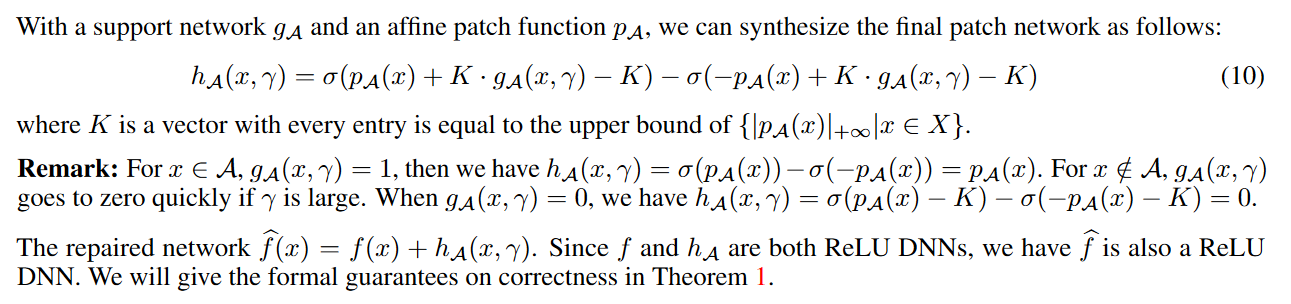
\includegraphics[width=\linewidth]{5.png}
	\end{figure}
\end{frame}

\begin{frame}
	\frametitle{Multi-Region Repairs}
	Observations:
	\begin{itemize}
		\item If Linregion $\mathcal{A}_1 \cap \mathcal{A}_2 \neq \emptyset$, 
		for any $x \in \mathcal{A}_1 \cap \mathcal{A}_2$,
		both $h_{\mathcal{A}_1}(x, \gamma)$ and $h_{\mathcal{A}_2}(x, \gamma)$ will alter the value of $f$ on $x$, 
		which will invalidate both repairs and cannot guarantee that the repaired DNN will meet the specification $\Phi$. \pause
		\item For$ \text { multi-region repair, we note }\left\{\mathcal{A}_l\right\}_{l=1,2, \ldots, L} \text { are all the buggy linear regions. }$
		\begin{enumerate}
			\item We compute the support network $g_{\mathcal{A}_i}(x,\gamma)$ and affine patch function $p_{\mathcal{A}_i}(x)$ for each $A_i$ in parallel.
			\item We repair $\mathcal{A}_i \cup \cdots \cup\mathcal{A}_L$ with $p_{\mathcal{A}_i}(x)-p_{\mathcal{A}_{i-1}}(x)$ in turn.
			\item We use $\max _{j \geq i}\left\{g_{\mathcal{A}_j}(x, \gamma)\right\}$ as characteristic function of $\mathcal{A}_i \cup \cdots \cup\mathcal{A}_L$
		\end{enumerate}
	\end{itemize} 
	
\end{frame}


\begin{frame}
	\frametitle{An example}
	\begin{figure}[htbp]
		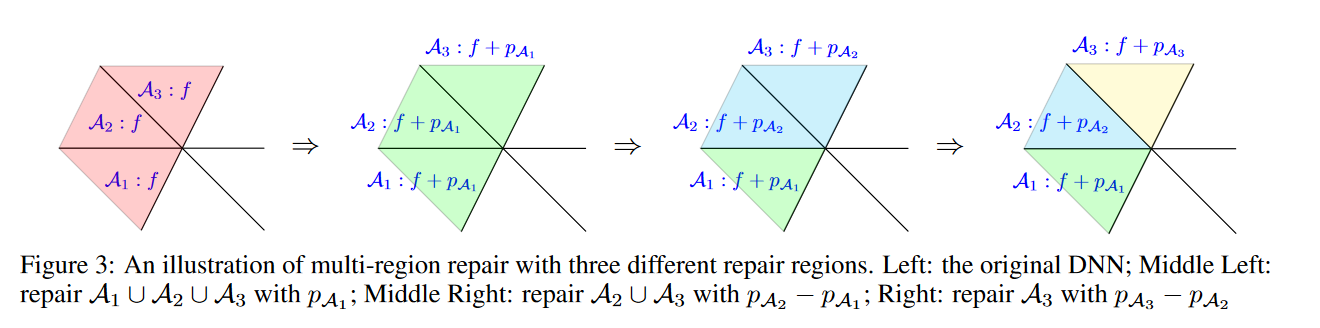
\includegraphics[width=\linewidth]{6.png}
	\end{figure}
\end{frame}

\begin{frame}
	\frametitle{Patch network of Multi-Region Repairs}
	\begin{equation}
		\begin{aligned}
		h(x, \gamma)= & \sum_l\left[\sigma\left(p_{\mathcal{A}_l}(x)-p_{\mathcal{A}_{l-1}}(x)+\max _{j \geq l}\left\{g_{\mathcal{A}_j}(x, \gamma)\right\} K_l-K_l\right)\right. \\
		& \left.-\sigma\left(-p_{\mathcal{A}_l}(x)+p_{\mathcal{A}_{l-1}}(x)+\max _{j \geq l}\left\{g_{\mathcal{A}_j}(x, \gamma)\right\} K_l-K_l\right)\right]
		\end{aligned}
	\end{equation}
	\qquad where $K_l$ is the upper bound of $\left\{\left|p_{\mathcal{A}_l}(x)-p_{\mathcal{A}_{l-1}}(x)\right|_{\infty} \mid x \in X\right\}$ and $p_{\mathcal{A}_0}(x)=0$.
\end{frame}

\begin{frame}
	\frametitle{Feature-Space Repairs}
	\begin{itemize}
		\item For large DNN, the huge number of linear constraints for one patch area $\mathcal{A}$ will pose a challenge to solving the resulting LP. \pause
		\item We can construct a patch network starting from an intermediate layer.
		\begin{itemize}
			\item Divide DNN $f$ into $f_1$ and $f_2$, i.e. $f=f_2 \circ f_1$.
			\item Add a patch network from the output space of $f_1$, which is a \textbf{feature space}.
		\end{itemize} \pause
		\item To repair the network in feature space, we can
		\begin{itemize}
			\item reduce the parameter overhead of the additional networks,
			\item and make the repair process more computation-friendly.
		\end{itemize} \pause
		\item We loses the locality guarantee in the input space but still preserves \textbf{locality in the feature space}.
	\end{itemize}
\end{frame}

\begin{frame}
	\frametitle{Algorithm}
	\begin{figure}[htbp]
		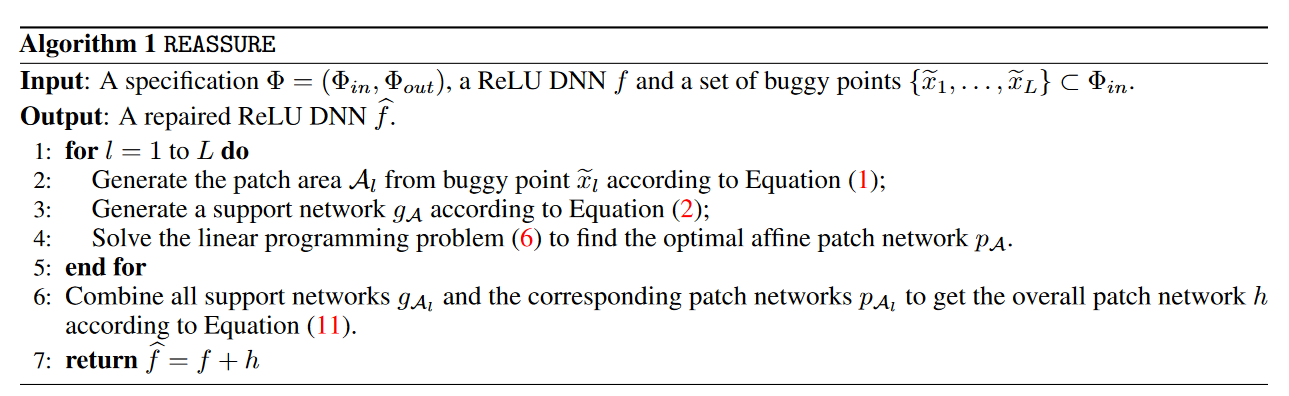
\includegraphics[width=\linewidth]{7.png}
	\end{figure}
\end{frame}

\section{Experiments}
\begin{frame}
	\frametitle{Notion}
	\begin{figure}[htbp]
		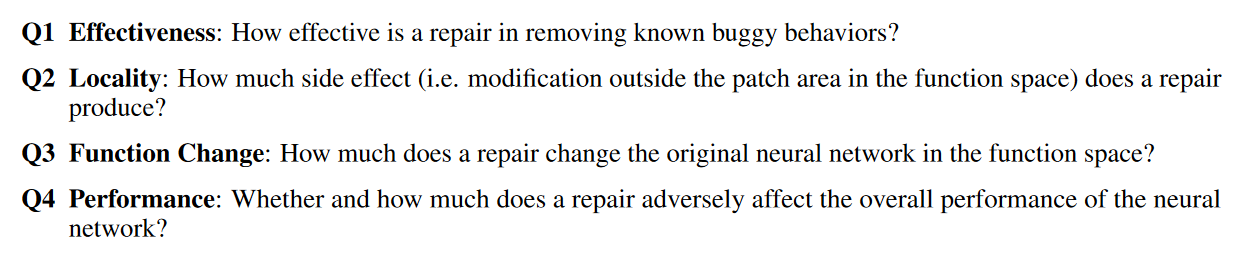
\includegraphics[width=\linewidth]{8.png}
	\end{figure}
\end{frame}

% \begin{frame}
% 	\frametitle{Evaluation criteria}
% 	\begin{itemize}
% 		\item Efficacy(E): \% of given buggy points or buggy linear regions that are repaired. \pause
% 		\item Norm Difference (ND): average norm ($L_\infty$ or $L_2$) difference between the original DNN and the repaired DNN on a set of inputs
% 		\begin{itemize}
% 			\item To measure how a repair \textbf{change} the original neural network on \textbf{function space}.
% 		\end{itemize} \pause
% 		\item Norm Difference on Patch Area (NDP): average norm ($L_\infty$ or $L_2$) difference between the original DNN and the repaired DNN on patch areas
% 		\begin{itemize}
% 			\item To calculate on random sampled points on patch areas or near the buggy points
% 			\item To measure the locality of a repair.
% 		\end{itemize} \pause
% 		\item Accuracy (Acc): accuracy on training or testing data to measure the extent to which a repair preserves the performance of the original neural network.
% 	\end{itemize}
% \end{frame}

\begin{frame}
	\frametitle{Point-wise Repairs: MNIST}
	\begin{figure}[htbp]
		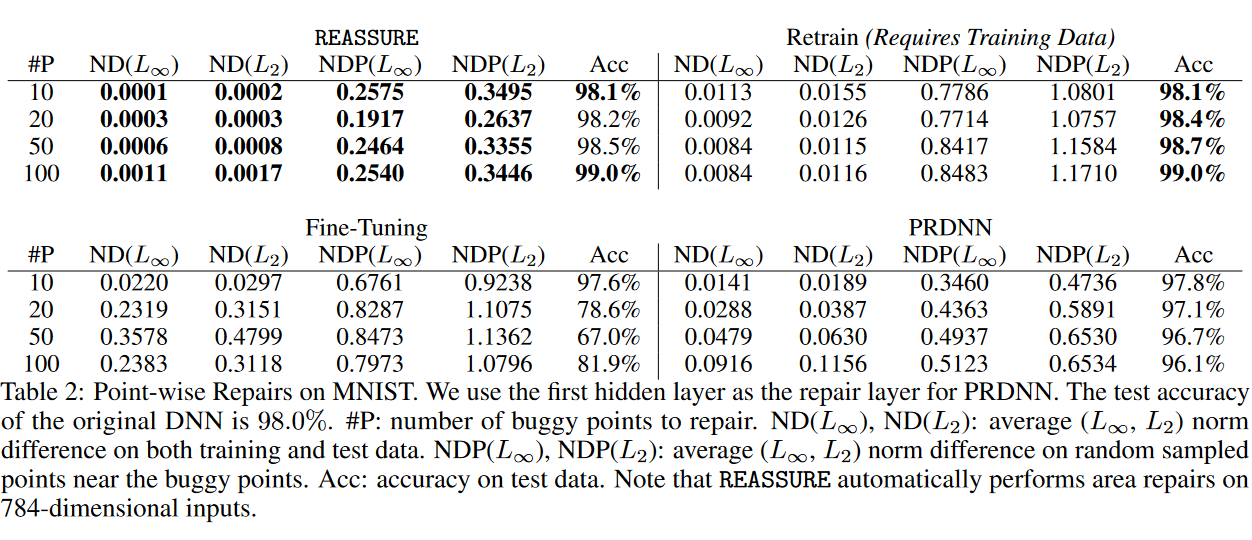
\includegraphics[width=\linewidth]{9.png}
	\end{figure}
\end{frame}

\begin{frame}
	\frametitle{Point-wise Repairs: MNIST}
	\begin{figure}[htbp]
		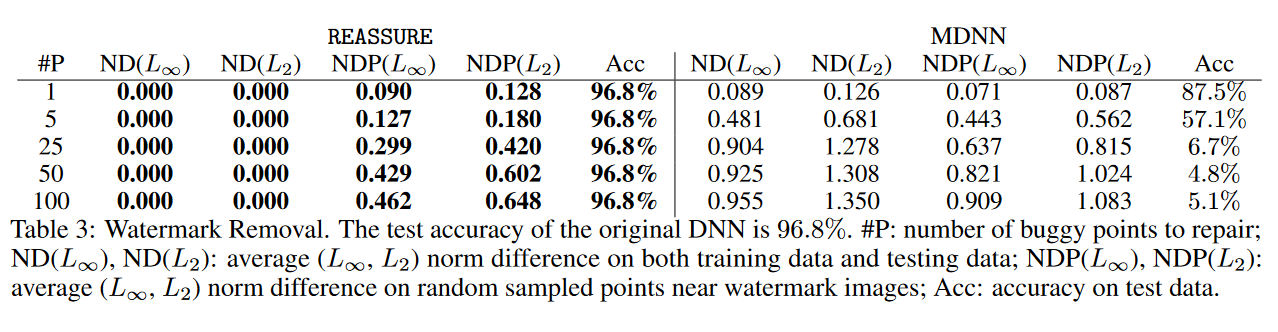
\includegraphics[width=\linewidth]{10.png}
	\end{figure}
\end{frame}

\begin{frame}
	\frametitle{Area Repairs: HCAS}
	\begin{itemize}
		\item Only compare with PRDNN \pause
		\item HCAS networks (simplified version of ACAS Xu)
		\begin{itemize}
			\item Each of them has an input layer with 3 nodes, 5 hidden layers with 25 nodes in each hidden layer, and a final output layer with 5 nodes. 
		\end{itemize} \pause
		\item We use the method from \textcolor{blue}{Girard-Satabin et al. [2021]} to compute all the linear regions for the network(87 buggy linear regions were found.) \pause
		\item We use Specification 1, which is similar to Property 5.
	\end{itemize}
\end{frame}

\begin{frame}
	\frametitle{Area Repairs: HCAS}
	\begin{figure}[htbp]
		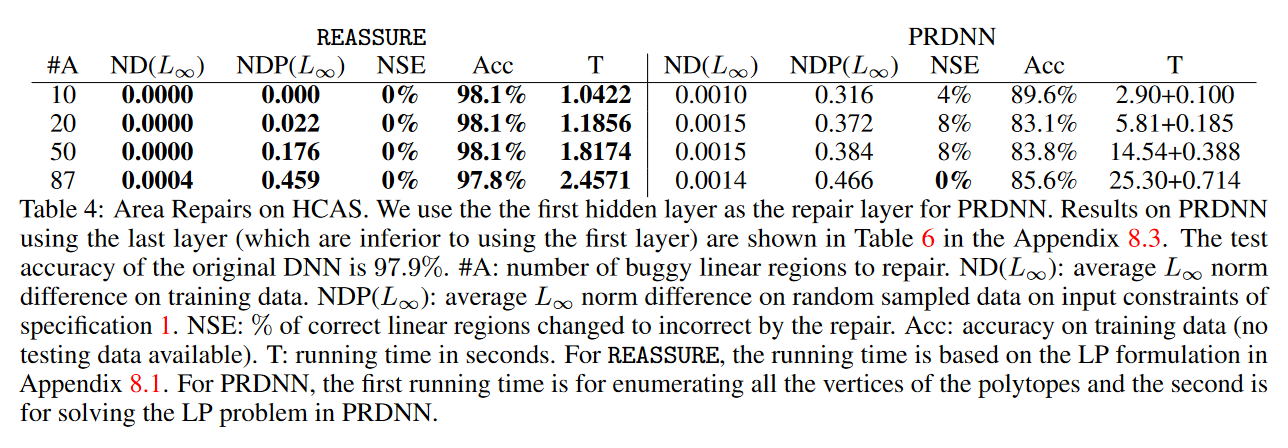
\includegraphics[width=\linewidth]{11.png}
	\end{figure}
\end{frame}

\begin{frame}
	\frametitle{Feature-Space Repairs: ImageNet}
	\begin{itemize}
		\item Only compare with PRDNN \pause
		\item They only consider 10 output classes(found on ImageNet-A \textcolor{blue}{Hendrycks et al. [2021]})\pause
		\item They slightly modified AlexNet by a multilayer perceptron with three hidden layers to simplify the evaluation.
		\item They construct the patch network starting from the third from the last hidden layers.
	\end{itemize}
\end{frame}

\begin{frame}
	\frametitle{Feature-Space Repairs: ImageNet}
	\begin{figure}[htbp]
		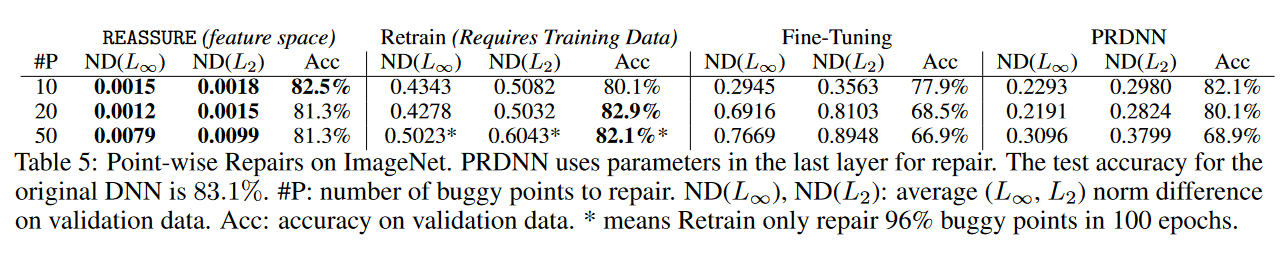
\includegraphics[width=\linewidth]{12.png}
	\end{figure}
\end{frame}

\section{Discussion}
\begin{frame}
	\frametitle{Parameter Overhead}
	\begin{itemize}
		\item REASSURE introduces new parameters for per repair region is in O(m|I|) \pause
		\item Use LP to check if a constraint is redundant.
		\begin{itemize} 
			\item For HCAS, only 3\% of the original 125 constraints after removing the redundant constraints
		\end{itemize} \pause
		\item Use feature-space repairs instead of input space
		\begin{itemize}
			\item 0.1\%(500k) of parameters from input space.
			\item trade off locality and parameter overhead.
			\item When the number of points or linear regions to repair becomes \textbf{large}, it may make sense to perform repairs in the feature space anyway for \textbf{better generalization}.
		\end{itemize}
	\end{itemize}
\end{frame}

%------------------------------------------------


%------------------------------------------------

%------------------------------------------------


%------------------------------------------------
\begin{frame}
\hfill
\center{\Huge{\calligra{\Huge{Thank you}}}}
\linespread{3}\selectfont
\end{frame}
%----------------------------------------------------------------------------------------
\end{document}